\chapter{Iteracion 4: Diseño final de hardware} % (fold)
\label{cha:iteracion_4}

\section{Introduccion} % (fold)
\label{sec:introduccion}

Nos propusimos poder duplicar la cantidad de recursos de la placa, ya que el principal problema era medir varios sensores de modo diferencial, con 8 entradas solo podriamos tener 4 sensores como maximo. Entonces decidimos poner dos microcontroladores a la placa. Pasar de 8 a 16 entradas analogicas y utilizar todas las entradas digitales. 
Para no agrandar el tamaño decidimos rediseñar la placa, y como primera medida la diseñamos para poder construirla doble capa.
En esta iteracion mostraremos como se realizo el diseño y la construccion de esta nueva placa.

% section introduccion (end)

\section{Requerimientos de la iteracion} % (fold)
\label{sec:requerimientos_de_la_iteracion}

\begin{itemize}
	\item La placa debe tener dos microcontroladores C8051f352.
	\item La placa debe tener 16 entradas analogicas.
	\item La placa debe tener 32 entradas digitales.
	\item La placa debe tener 2 salidas seriales. 
\end{itemize}

% section requerimientos_de_la_iteracion (end)

\section{Desarrollo} % (fold)
\label{sec:desarrollo}

\subsection{Diseño Esquematico}
\label{sub: diseño_esquematico2}

Para simplificar la explicación del diagrama, lo que haremos en esta sección es dividir el circuito entero en subcircuitos mas simples.

\subsubsection{Entradas Analogicas}
\label{subsub: entradas_analogicas2}

Las entradas analogicas con sus filtros se mantuvieron exactamente igual que en el diseño de la primera placa. Para cada una de las entradas se le colocaria un filtro pasa-bajo RC como se muestra en la figura \ref{fig:esquematicoFiltro}.

Mostramos en la figura \ref{fig:esquematicoFiltro2} como quedan todas las entradas analógicas de un solo chip (en el otro es exactamente igual), podemos ver 8 entradas analogicas, cada una con su respectivo filtro. Ademas podemos observar 2 pines llamados PINHD_AGND_2, son dos accesos a la masa digital para aquellos sensores que necesiten estar referenciado a masa (colocamos dos masa analogicas para cada uno de los chips).

Del lado derecho del microcontrolador hay dos entradas denominadas VREF+ y VREF-, que nos sirven para manejar los niveles de tension de referencia para la conversion que usara el ADC.

\begin{figure}
\centering
  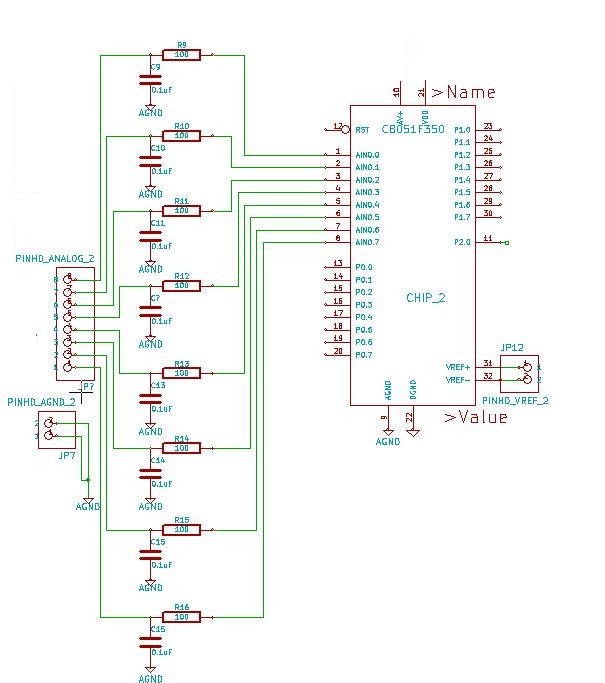
\includegraphics[width=1.10\textwidth, height = 12cm]{esquematicoFiltro2}
  \caption{Esquemático del Circuito Completo de entradas analogicas.}\label{fig:esquematicoFiltro2}
\end{figure}

% subsubsection entradas_analogicas2 (end)

\subsubsection{Circuito de entradas Digitales}
\label{subsub:entradas_digitales}

Como podemos ver en la figura \ref{fig:esquematicoDigital2} colocamos 16 entradas/salidas digitales para el microcontrolador. Cada chip tiene las mismas 16 entradas.

\begin{figura}	
\centering
  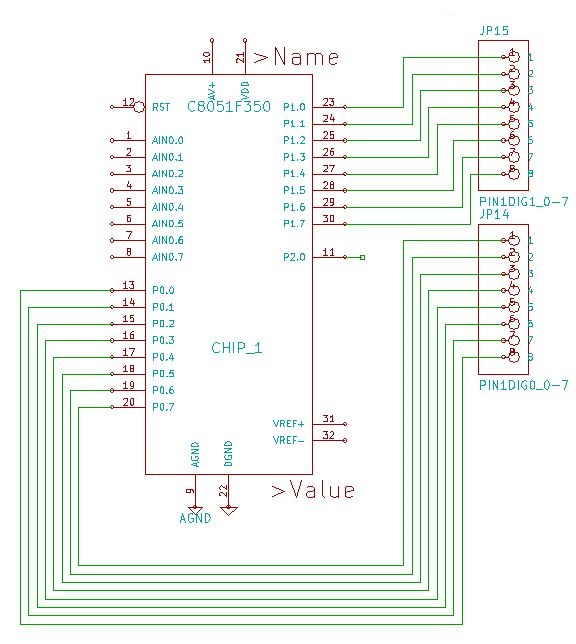
\includegraphics[width=1.10\textwidth, height = 12cm]{esquematicoDigital2}
  \caption{Esquemático del Circuito Completo de entradas/salidas digitales.}\label{fig:esquematicoDigital2}
\end{figure}


% subsubsection entradas_digitales (end)

\subsubsection{Circuito Salida Serial}
\label{subsub:salida_serial2}

La idea de tener una placa a la que se conecten varios sensores analógicos y digitales es que se pueda colocar el lugares remotos, por lo que decidimos que la salida serial deje de ser RS-232 y colocarle dos salidas seriales nivel TTL con un RX y un TX para cada microcontrolador, ademas colocando éste tipo de salida se ahorra mucho espacio, así pudimos reducir el tamaño de la placa. Las salidas seriales se encuentran conectadas directamente en los pines de salidas dijitales P0.4 (Tx) y P0.5(Rx).

% subsubsection salida_serial2 (end)

\subsubsection{Circuito para Debugger y Programación} % (fold)
\label{subsub:debugger_programacion2}

Para programar cada uno de los microcontroladores en principio se penso en colocar dos entradas para el debugger de SiliconLabs, pero nos consumia mucho espacio y el cambio para programar uno y otro se hubiera hecho molesto. Por lo que decidimos poner uno solo, y utilizarlo para los dos microcontroladores, con un jumper de tres pines, para tener la opcion de elegir que micro programar.
En la figura \ref{fig:esquematicoDebugger2} vemos en uno de los C8051f352 como queda conectado el modulo de debugger/programacion.

\begin{figura}	
\centering
  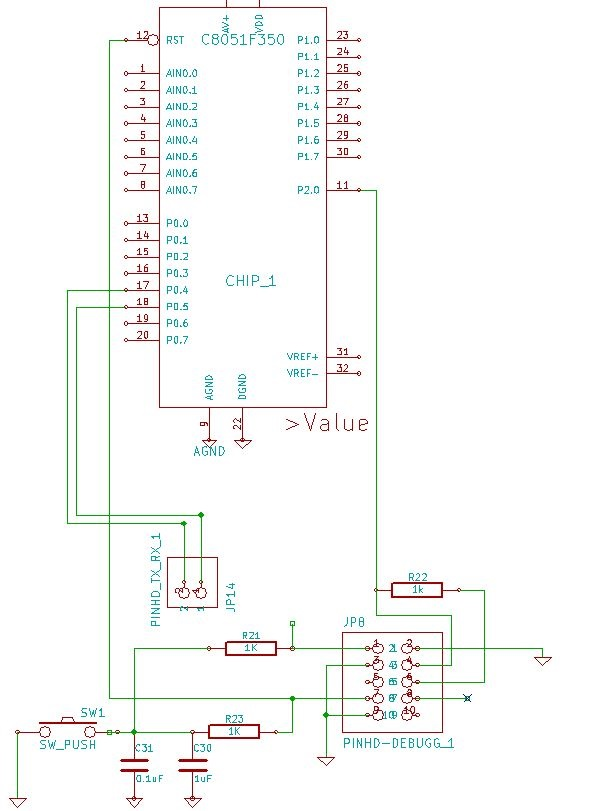
\includegraphics[width=1.10\textwidth, height = 12cm]{esquematicoDebugger2}
  \caption{Esquemático del Circuito Completo para la programacion de los microcontroladores de la placa.}\label{fig:esquematicoDebugger2}
\end{figure}


% subsection debugger_programacion2 (end)

\subsubsection{Circuito de Potencia}
\label{subsub: circuito_potencia2}

Para el circuito de potencia hicimos lo mismo que con el debugger, colocamos una sola entrada y un solo regulador para toda la placa y alimentar asi los dos microcontroladores, 

%subsection circuito_potencia2 (end)

% subsection diseño_esquematico2 (end)

% section desarrollo (end)

\section{Pruebas} % (fold)
\label{sec:pruebas}

% section pruebas (end)

\section{Resultados} % (fold)
\label{sec:resultados}

% section resultados (end)

% chapter iteracion_4 (end)